\documentclass[11pt,a4paper]{article}

\usepackage{graphicx}
\usepackage{amsmath}
\usepackage{hyperref}
\usepackage{listings}
\usepackage{geometry}

\geometry{margin=2.5cm}

\title{BioTrajectoryAnalysis\\
User Manual\
Version 1.0}

\author{Danilo Roccatano\\
School of Mathematics and Physics\\
University of Lincoln}

\date{\today}

\begin{document}

\maketitle

\tableofcontents

\section{Introduction}

BioTrajectoryAnalysis is an open-source collection of Python tools for the extraction and quantitative analysis of biological trajectories from video recordings.

The software combines computer vision, automated tracking, and statistical-physics descriptors to characterize motion patterns in biological systems. The first module included in the project, \texttt{AntTrajectoryAnalysis}, was developed for the study of ant foraging trajectories, but the methodology can be extended to other organisms such as protozoa, rotifers, nematodes, and slugs.

The software consists of two main programs:

\begin{enumerate}
\item \texttt{AntTracking\_V1.0.py}  for trajectory extraction.
\item \texttt{AntTrajectoryAnalysis\_V1.0.py} for statistical analysis.
\end{enumerate}

\section{Software Architecture}

BioTrajectoryAnalysis is organized as a modular framework composed of independent tools for trajectory extraction, trajectory analysis, and visualization.

The current release includes:

\begin{enumerate}
\item \texttt{AntTracking\_V1.0.py}
\item \texttt{AntTrajectoryAnalysis\_V1.0.py}
\end{enumerate}

The modular architecture allows future extensions dedicated to other biological systems, including protozoa, rotifers, nematodes, insects, and small aquatic organisms.

\vspace{0.5cm}

The overall workflow is:

\begin{center}
Video Acquisition

$\downarrow$

Object Detection

$\downarrow$

Trajectory Reconstruction

$\downarrow$

Statistical Analysis

$\downarrow$

Scientific Figures and Reports
\end{center}


\section{Workflow}

The typical workflow is:

\begin{center}
Video Recording

$\downarrow$

Trajectory Extraction

$\downarrow$

CSV Trajectory File

$\downarrow$

Statistical Analysis

$\downarrow$

Figures and Reports
\end{center}

\section{Installation}

The software requires:

\begin{itemize}
\item Python 3.10 or newer
\item OpenCV
\item NumPy
\item Pandas
\item SciPy
\item Matplotlib
\item scikit-learn
\end{itemize}

The required packages can be installed using:

\begin{verbatim}
pip install -r requirements.txt
\end{verbatim}

section{Coordinate System}

Video images are internally represented according to the OpenCV image convention, where the origin is located at the upper-left corner of the image.

For all statistical analyses and graphical outputs, coordinates are transformed into a Cartesian coordinate system:

\begin{itemize}
\item origin located at the lower-left corner,
\item x-axis increasing from left to right,
\item y-axis increasing from bottom to top.
\end{itemize}

This transformation facilitates comparison with standard physical and mathematical coordinate systems.


\section{Trajectory Extraction}

\subsection{Overview}

The program \texttt{AntTracking\_V1.0.py}  extracts trajectories from video recordings.

The program can:

\begin{itemize}
\item Select a region of interest (ROI)
\item Detect moving organisms
\item Filter detections by size and shape
\item Reconstruct trajectories
\item Convert pixel coordinates into physical units
\item Save trajectory data
\end{itemize}

\subsection{Basic Usage}

\begin{verbatim}
python AntTracking_V1.0.py video.mov
\end{verbatim}

\subsection{Example}

\begin{verbatim}
python AntTracking_V1.0.py video.mov
    --threshold 18
    --min-area 6
    --max-area 250
    --output tracking_results
\end{verbatim}

\subsection{Important Parameters}

\begin{description}

\item[threshold]
Motion detection threshold.

\item[min-area]
Minimum contour area accepted as a valid object.

\item[max-area]
Maximum contour area accepted as a valid object.

\item[max-distance]
Maximum distance used to associate detections between frames.

\item[max-gap]
Maximum number of missing frames allowed before terminating a track.

\item[merge-distance]
Distance used to merge nearby detections.

\end{description}

\section{Output Files}

Typical output includes:

\begin{itemize}
\item \texttt{ant\_tracks.csv}
\item \texttt{config.json}
\item diagnostic images
\item tracking statistics
\end{itemize}

\section{Trajectory Data Format}

Trajectory data are stored in CSV format.

A typical file contains:

\begin{verbatim}
track_id,frame,x,y
1,0,123.4,201.7
1,1,124.2,202.3
1,2,125.0,203.1
\end{verbatim}

where:

\begin{description}
\item[track\_id] trajectory identifier.
\item[frame] video frame number.
\item[x] horizontal coordinate.
\item[y] vertical coordinate.
\end{description}

Coordinates may be expressed either in pixels or physical units depending on the calibration settings.

\section{Trajectory Analysis}

\subsection{Overview}

The program \texttt{AntTrajectoryAnalysis\_V1.0.py} computes statistical descriptors from the extracted trajectories.

The software performs:

\begin{itemize}
\item Convex hull analysis
\item Monte Carlo area estimation
\item Occupancy mapping
\item Principal Component Analysis (PCA)
\item Mean Squared Displacement (MSD)
\item Straightness analysis
\item Fractal dimension estimation
\end{itemize}

\subsection{Basic Usage}

\begin{verbatim}
python AntTrajectoryAnalysis_V1.0.py
    ant_tracks.csv
\end{verbatim}

\subsection{Example}

\begin{verbatim}
python AntTrajectoryAnalysis_V1.0.py
    ant_tracks.csv
    --cm-per-pixel 0.02
    --output analysis_results
\end{verbatim}

\section{Generated Figures}

The analysis program produces several publication-quality figures.

\subsection{Spatial Exploration and Anisotropy}

Shows:

\begin{itemize}
\item trajectory map
\item convex hull
\item PCA axes
\item whitened coordinates
\end{itemize}

\subsection{Occupancy Maps}

Shows spatial utilization of the explored region.

\subsection{Monte Carlo Area Estimation}

Illustrates the Monte Carlo estimate of the explored area.

\subsection{Trajectory Statistics}

Includes:

\begin{itemize}
\item Mean Squared Displacement
\item Straightness distributions
\item Additional trajectory descriptors
\end{itemize}

\section{Statistical Descriptors}



\subsection{Explored Area}

Estimated using the convex hull of all recorded positions.

\subsection{Occupancy Maps}

Quantify how frequently different regions are visited.

\subsection{Principal Component Analysis}

Measures spatial anisotropy.

\subsection{Mean Squared Displacement}

Characterizes transport properties.

\subsection{Straightness}

Measures path tortuosity.

\subsection{Fractal Dimension}

Quantifies the complexity and space-filling properties of trajectories.


\section{Mathematical Background}

\subsection{Mean Squared Displacement}

The Mean Squared Displacement (MSD) is defined as

\begin{equation}
MSD(\tau)=
\left<
|\mathbf r(t+\tau)-\mathbf r(t)|^2
\right>.
\end{equation}

For many biological systems, the MSD follows a power law
\begin{equation}
MSD(\tau)\propto\tau^\beta.
\end{equation}

The exponent $\beta$ characterizes the transport regime:

\begin{itemize}
\item $\beta<1$ : subdiffusive motion,
\item $\beta=1$ : normal diffusion,
\item $\beta>1$ : superdiffusive motion.
\end{itemize}

\subsection{Principal Component Analysis}

Principal Component Analysis (PCA) determines the principal axes of spatial exploration.

The covariance matrix
\begin{equation}
C= \begin{bmatrix}
\sigma_x^2 & \sigma_{xy}\\
\sigma_{xy} & \sigma_y^2
\end{bmatrix}
\end{equation}

is diagonalized to obtain eigenvalues $\lambda_1$ and $\lambda_2$.

The anisotropy ratio is defined as
\begin{equation}
A=\frac{\lambda_1}{\lambda_2}.
\end{equation}

Values significantly larger than unity indicate strongly anisotropic exploration.

\subsection{Convex Hull Area}

The explored region is estimated from the convex hull enclosing all recorded positions.

The convex hull provides a simple estimate of the maximum explored area.

\subsection{Monte Carlo Area Estimation}

A Monte Carlo procedure is used to estimate the explored area.

Random points are generated inside the bounding box and classified according to whether they fall inside or outside the convex hull.

The area estimate is
\begin{equation}
A_{MC}= A_{box} \frac{N_{inside}} {N_{total}}.
\end{equation}

Confidence intervals are computed from the associated binomial statistics.

\subsection{Fractal Dimension}

The fractal dimension provides a measure of trajectory complexity and space-filling behavior.

Values approaching one correspond to nearly straight trajectories, whereas larger values indicate increasingly tortuous paths.

\section{Output Directory Structure}

A typical tracking run generates:

\begin{verbatim}
tracking_results/

  |----- ant_tracks.csv
  |----- config.json
  |----- tracking_statistics.txt
  |-----  diagnostic_images/
\end{verbatim}

A typical analysis run generates:

\begin{verbatim}
analysis_results/

  |-----  analysis_report.txt
  |-----  analysis_results.json
  |----- spatial_exploration_anisotropy.pdf
  |----- density_heatmap.pdf
  |----- trajectory_statistics.pdf
  |-----  monte_carlo_area.pdf
\end{verbatim}

\section{Applications}

Although originally developed for ant foraging studies, the software can be applied to a broad range of biological systems.

Examples include:

\begin{itemize}
\item Ants and social insects
\item Protozoa
\item Rotifers
\item Nematodes
\item Slugs and snails
\item Small aquatic organisms
\item Experimental active-matter systems
\item Artificial agents and robotic swarms
\end{itemize}

The software is particularly suitable for educational projects, movement ecology studies, and statistical-physics investigations of biological motion.

\section{Worked Example}

This section illustrates a complete analysis starting from a trajectory file generated by the tracking program.

\subsection{Running the analysis}

Run the tracking script using the given \texttt{config.json} file.

\begin{verbatim}
python3 ../tracking/AntTracking_V1.0.py SampleVideo.mov --config config.json --display --output tracking_results 
\end{verbatim}

\begin{figure}[ht]
\centering
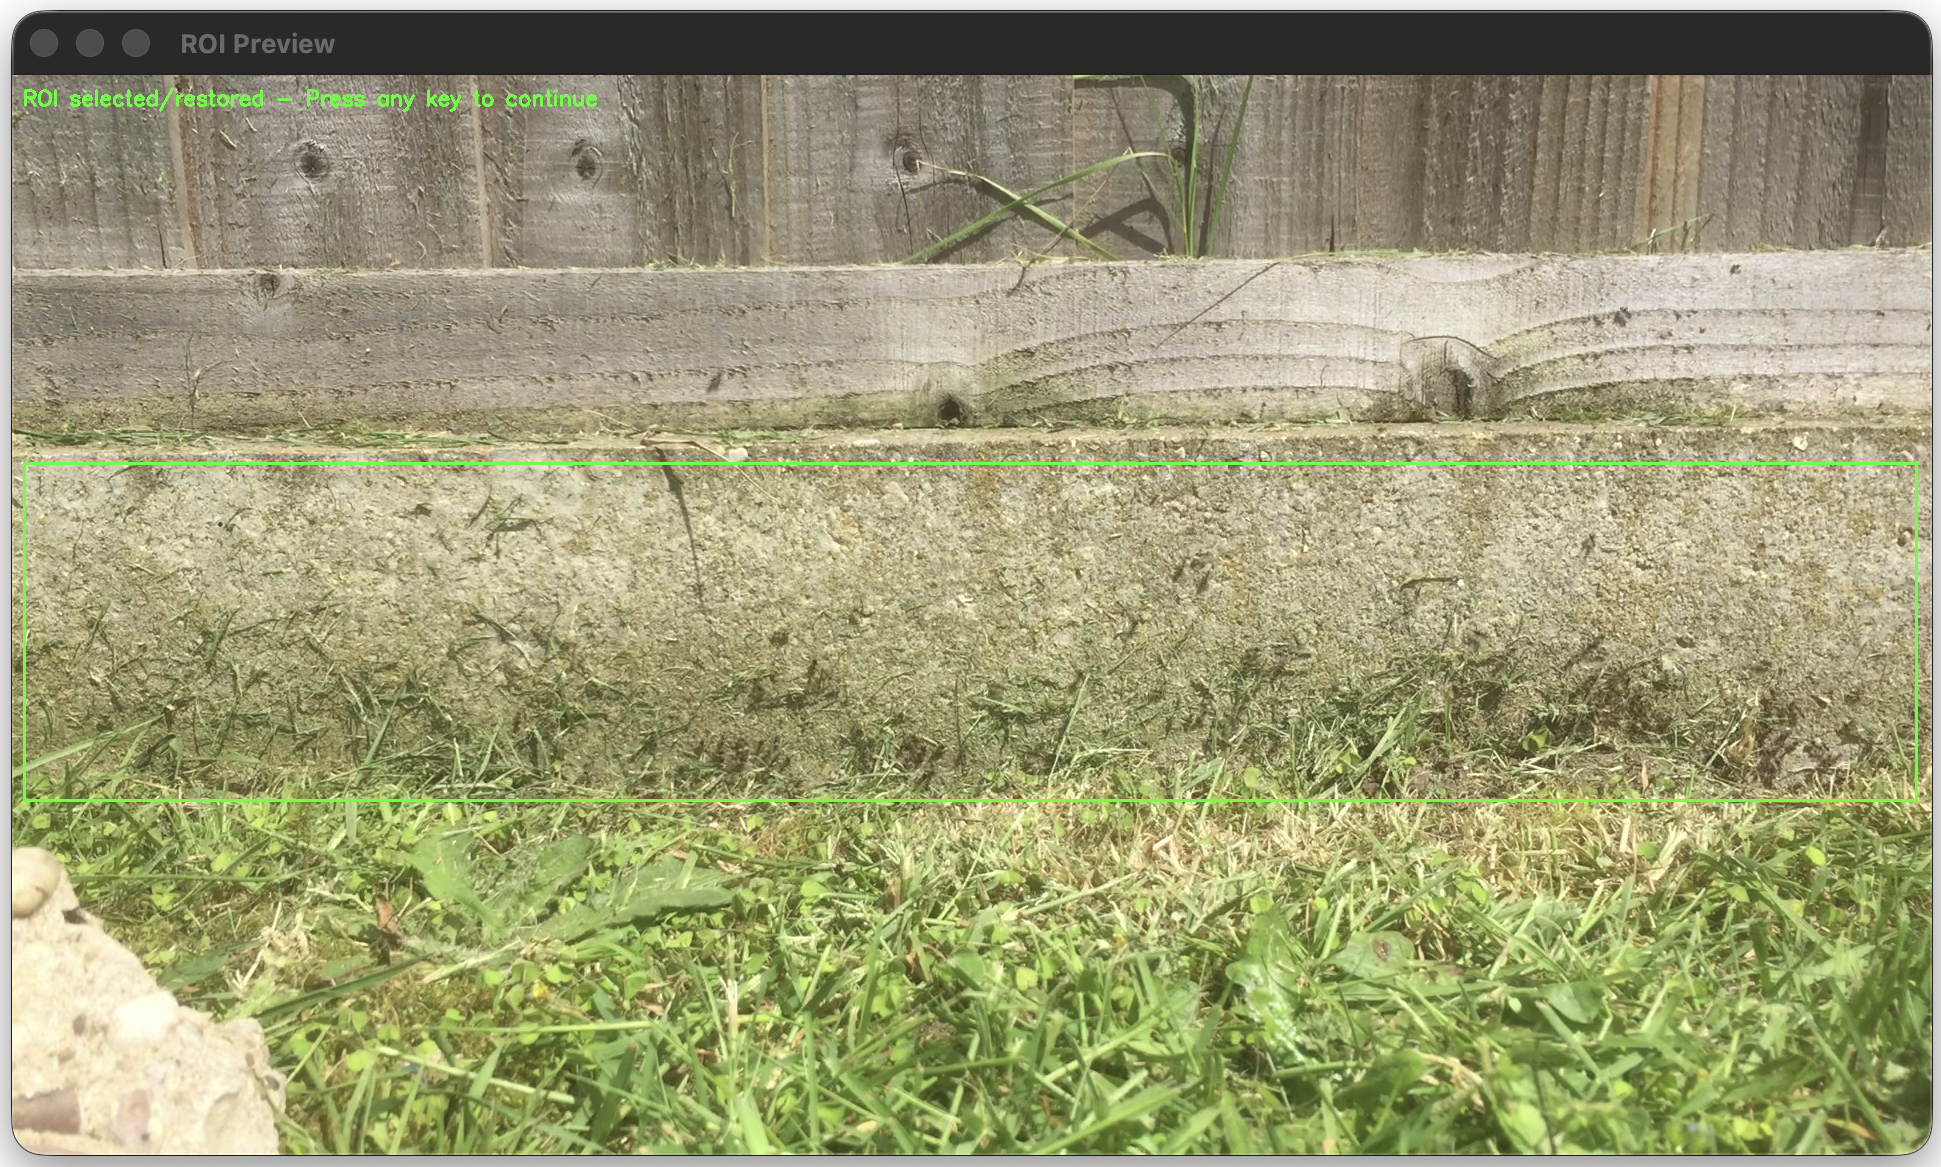
\includegraphics[width=0.85\textwidth]{figures/Tracking_Screenshot0.png}

\vspace{0.5cm}

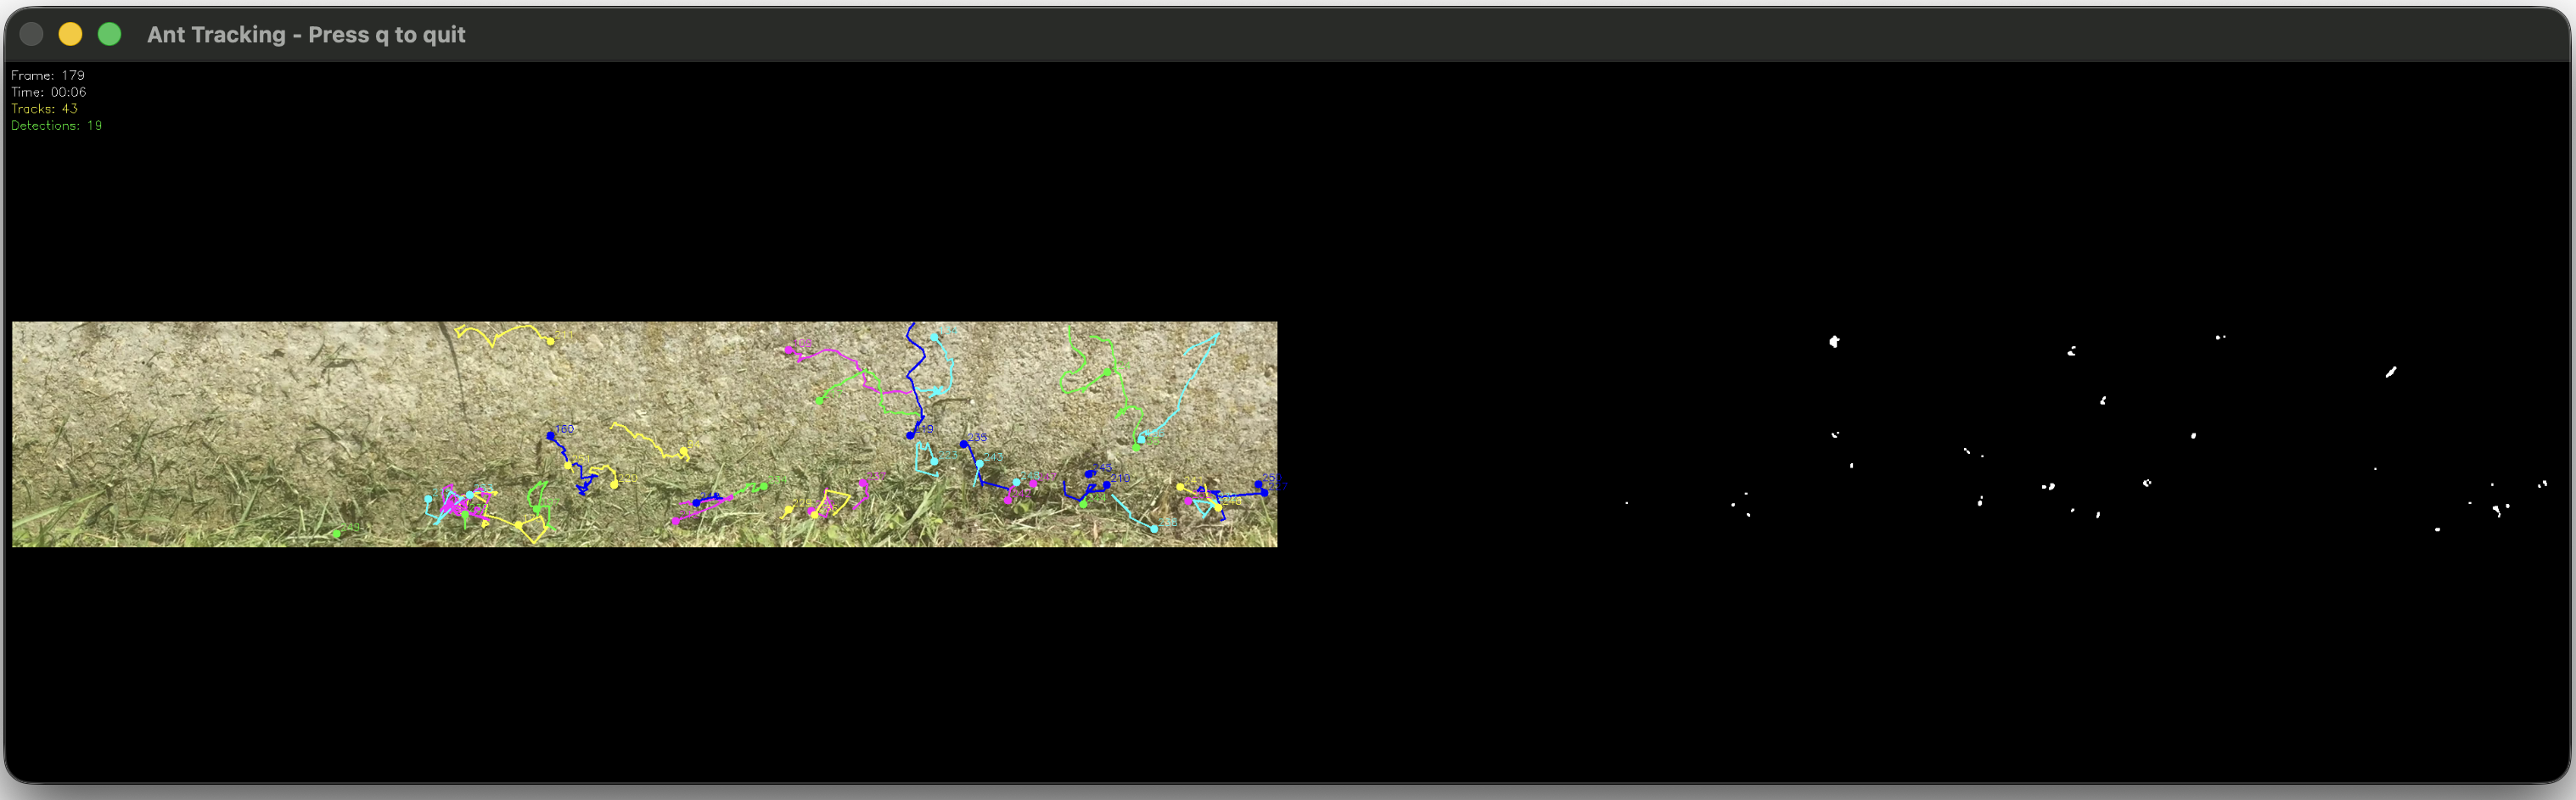
\includegraphics[width=0.85\textwidth]{figures/Tracking_Screenshot1.png}

\caption{
Tracking software interface. \textbf{Top:} Selection of the region of interest (ROI), indicated by the green rectangle. The ROI coordinates are stored in the \texttt{config.json} file and can be reused for subsequent analyses. \textbf{Bottom:} After confirming the ROI selection, the program begins the analysis. Moving ants are detected and tracked, and individual trajectories are displayed using different colours.
}
\label{fig:tracking_interface}
\end{figure}
After tracking a video, the file \texttt{ant\_tracks.csv} is saved in the output directory. The trajectory-analysis program can be run using:

\begin{verbatim}
python3 ../analysis/AntTrajectoryAnalysis_V1.0.py tracking_results/ant_tracks.csv
\end{verbatim}

The program loads the trajectory file, identifies the coordinate units and track columns, computes the statistical descriptors, and generates figures and report files.

A typical output is:

\begin{verbatim}
ANT TRAJECTORY ANALYSIS
Spatial exploration | Monte Carlo area | PCA anisotropy | stochastic descriptors
================================================================================
Loading: tracking_results/ant_tracks.csv
Loaded 23,708 positions
Coordinate unit: cm
cm_per_pixel: 0.027607362
ID column: track_id; frame column: frame
Generating figures...
\end{verbatim}

\subsection{Example analysis report}

The program generates a text report summarizing the main descriptors. For example:

\begin{verbatim}
1. SPATIAL EXPLORATION AND MONTE CARLO AREA
Convex hull area: 454.3026 cm^2
Circularity index: 0.4188
Monte Carlo area: 453.3648 cm^2
Monte Carlo 95% CI: [452.3860, 454.3437] cm^2

2. PCA ANISOTROPY
Anisotropy ratio lambda1/lambda2: 32.2926
Principal orientation: 179.25 degrees
Explained variance PC1: 97.00%

3. STOCHASTIC TRAJECTORY DESCRIPTORS
MSD exponent beta: 1.3492
Mean straightness: 0.4245
Fractal dimension D: 1.6850
\end{verbatim}

\subsection{Generated output files}

The analysis creates an output directory named \texttt{ant\_trajectory\_biophysics\_analysis} containing:

\begin{itemize}
\item \texttt{analysis\_report.txt}
\item \texttt{analysis\_results.json}
\item \texttt{spatial\_exploration\_anisotropy.pdf}
\item \texttt{density\_heatmap.pdf}
\item \texttt{trajectory\_statistics.pdf}
\item \texttt{monte\_carlo\_area.pdf}
\end{itemize}

\subsection{Example figures}

The generated figures summarize different aspects of the trajectory dataset.

\begin{figure}[ht]
\centering
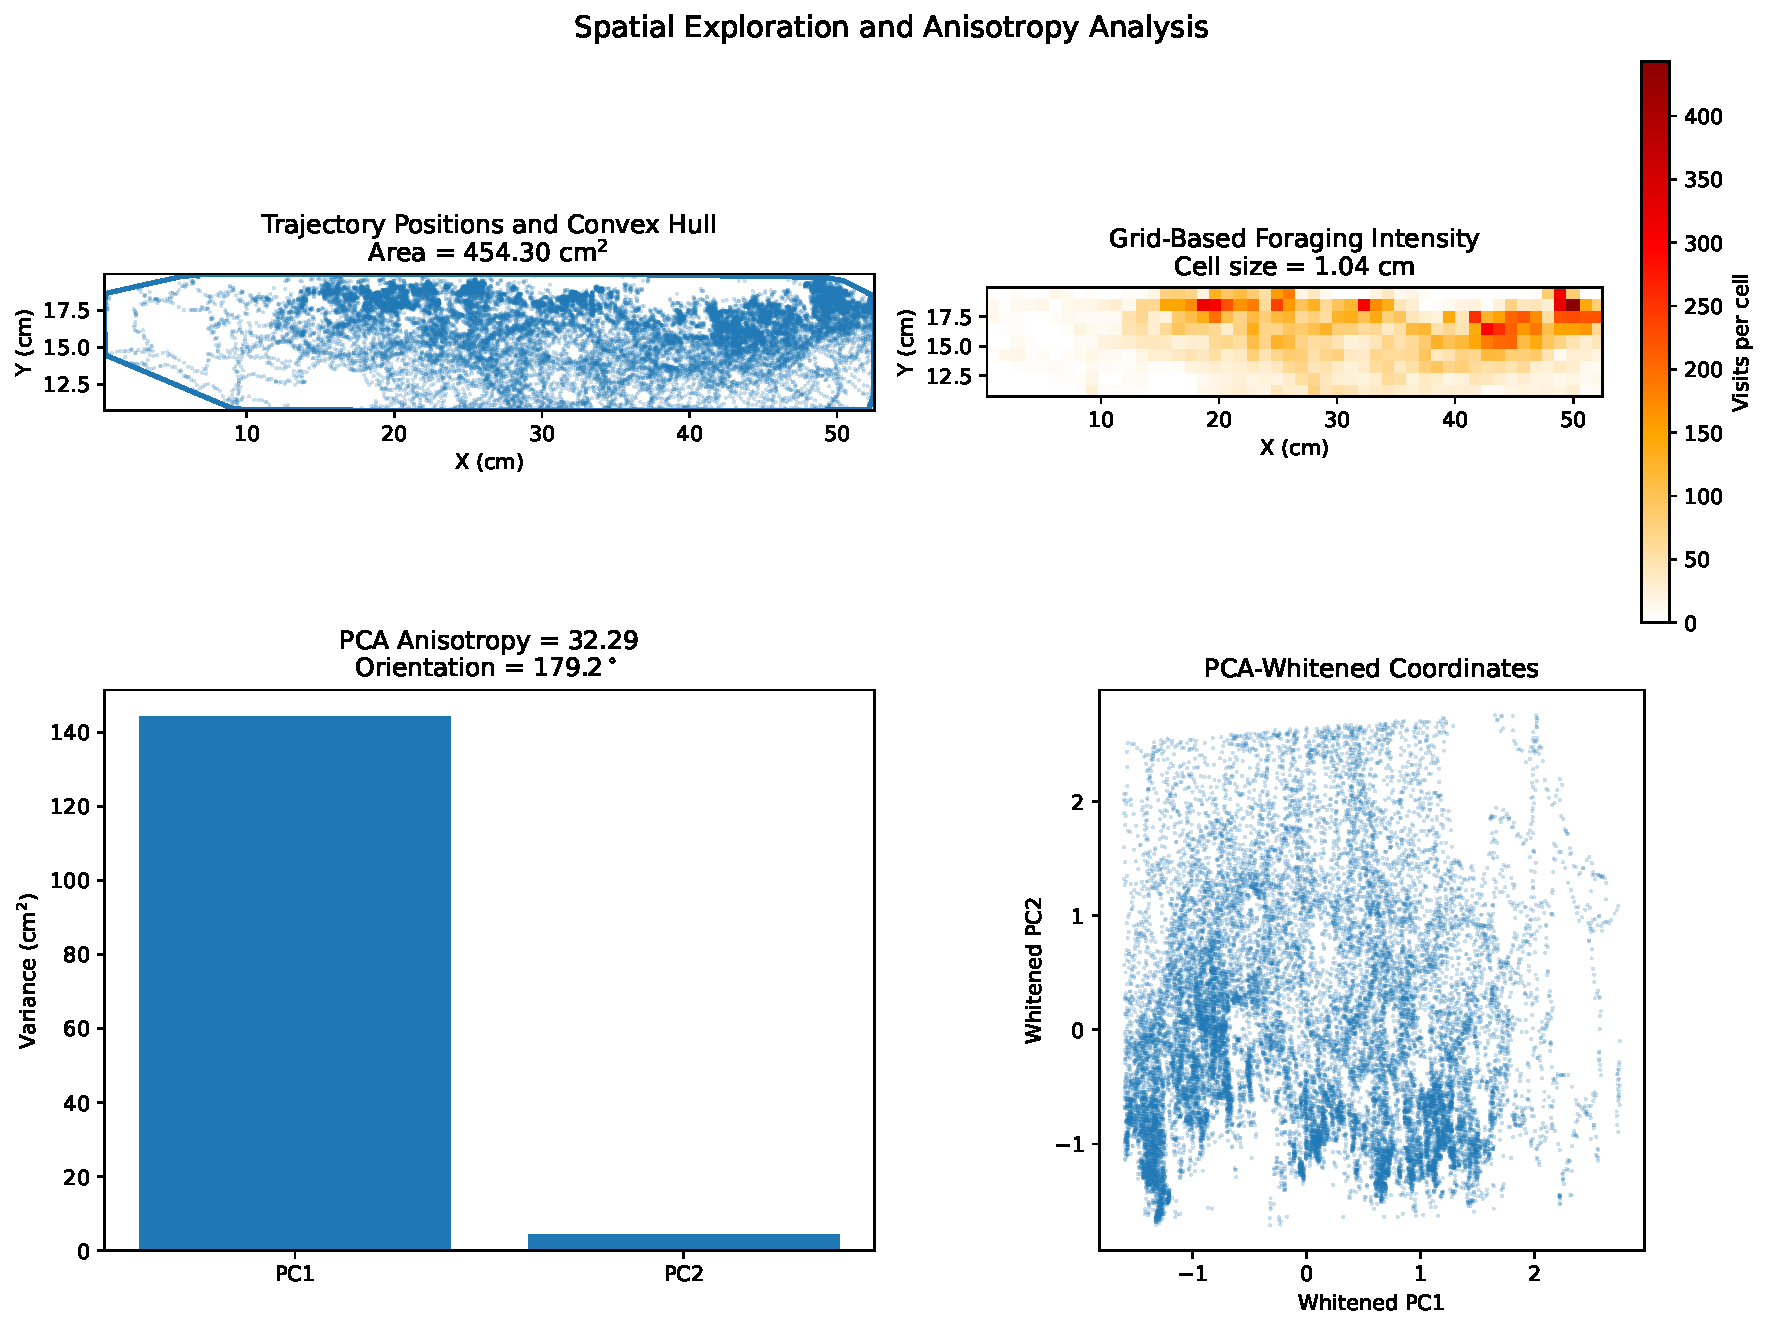
\includegraphics[width=0.85\textwidth]{figures/spatial_exploration_anisotropy.pdf}
\caption{Example output showing tracked positions, convex hull, and PCA-based anisotropy analysis.}
\end{figure}

\begin{figure}[ht]
\centering
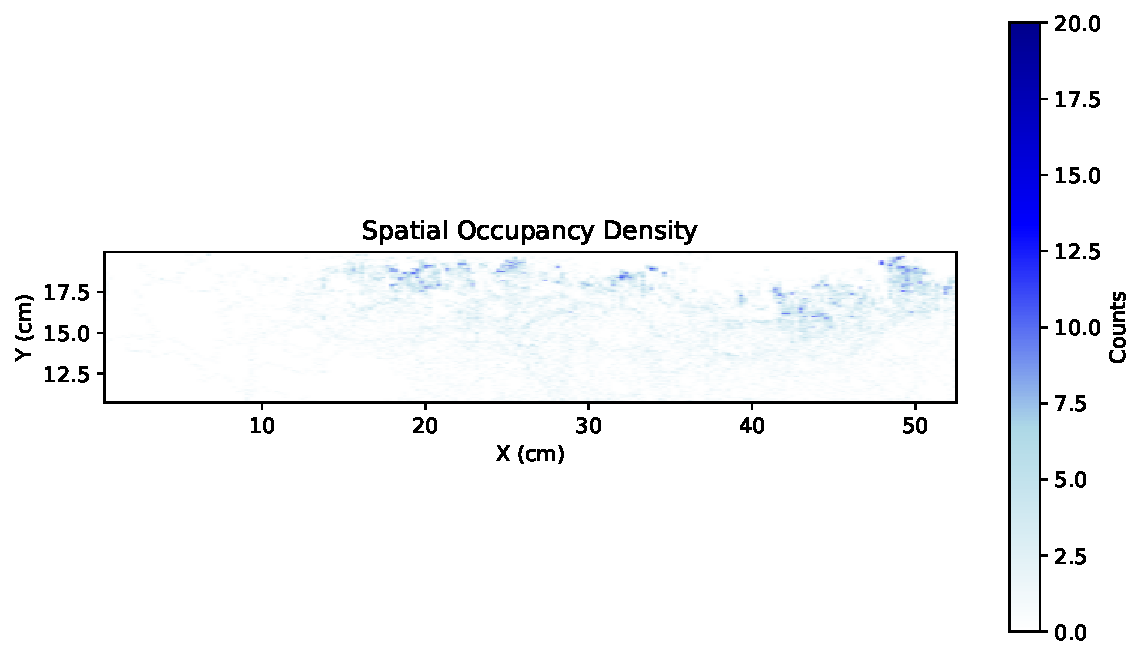
\includegraphics[width=0.85\textwidth]{figures/density_heatmap.pdf}
\caption{Example spatial occupancy map generated from the tracked ant positions.}
\end{figure}

\subsection{Interpretation}

In this example, the trajectory distribution is strongly anisotropic, with an anisotropy ratio of approximately 32. The convex-hull and Monte Carlo area estimates are in close agreement, showing that the Monte Carlo method provides a reliable estimate of the explored spatial domain. The MSD exponent is larger than one, indicating superdiffusive motion, while the fractal dimension provides a measure of the space-filling character of the trajectories.

\section{Limitations}

The current implementation assumes two-dimensional motion within the imaging plane.

Tracking accuracy may be affected by:

\begin{itemize}
\item poor image contrast,
\item severe object overlap,
\item strong illumination changes,
\item out-of-plane motion.
\end{itemize}

Careful calibration and video acquisition conditions are therefore recommended.

\section{Citation}

If you use this software in academic work, please cite the associated publication and the BioTrajectoryAnalysis repository.

\section{Future Developments}

Planned developments include:

\begin{itemize}
\item machine-learning assisted tracking,
\item multi-object interaction analysis,
\item three-dimensional trajectory reconstruction,
\item automated behavioral classification,
\item support for additional biological systems.
\end{itemize}

\section{License}

This software is distributed under the MIT License.

\end{document}

